% Band-capping geometry, drawn in a 2D slice of the residual stream. All
% coordinates are schematic; they are chosen so that the picture is readable,
% not measured from the experiments. The band is the slab of activations whose
% projection on \hat c_l lies within \beta \lVert c_l \rVert of p_l's, so its
% edges run perpendicular to c_l.
% Include with % Band-capping geometry, drawn in a 2D slice of the residual stream. All
% coordinates are schematic; they are chosen so that the picture is readable,
% not measured from the experiments. The band is the slab of activations whose
% projection on \hat c_l lies within \beta \lVert c_l \rVert of p_l's, so its
% edges run perpendicular to c_l.
% Include with % Band-capping geometry, drawn in a 2D slice of the residual stream. All
% coordinates are schematic; they are chosen so that the picture is readable,
% not measured from the experiments. The band is the slab of activations whose
% projection on \hat c_l lies within \beta \lVert c_l \rVert of p_l's, so its
% edges run perpendicular to c_l.
% Include with % Band-capping geometry, drawn in a 2D slice of the residual stream. All
% coordinates are schematic; they are chosen so that the picture is readable,
% not measured from the experiments. The band is the slab of activations whose
% projection on \hat c_l lies within \beta \lVert c_l \rVert of p_l's, so its
% edges run perpendicular to c_l.
% Include with \input{figures/steering_geometry}; needs tikz and amsmath.
\begin{figure}[t]
  \centering
  \footnotesize
  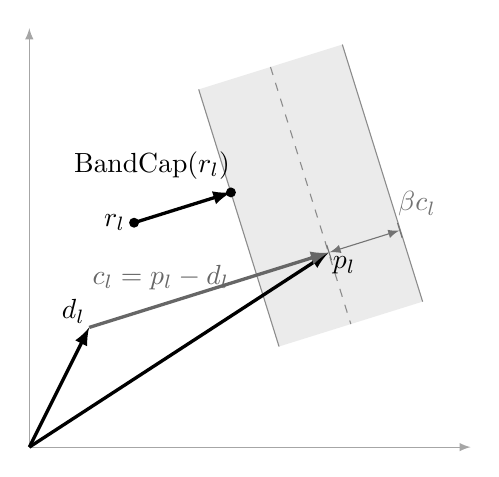
\begin{tikzpicture}[x=0.95cm, y=0.95cm, >=latex, line join=round]
    % Axes of the 2D slice.
    \draw[->, black!35] (0,0) -- (5.9,0);
    \draw[->, black!35] (0,0) -- (0,5.6);

    % The band: a slab perpendicular to c_l, centred on p_l's projection.
    \fill[black!8] (2.264,4.782) -- (4.184,5.382) -- (5.258,1.945) --
                   (3.338,1.345) -- cycle;
    \draw[black!45] (2.264,4.782) -- (3.338,1.345);
    \draw[black!45] (4.184,5.382) -- (5.258,1.945);
    % Centre line of the band: p_l's own projection on \hat c_l.
    \draw[dashed, black!45] (3.224,5.082) -- (4.298,1.645);

    % The two published vectors and their difference.
    \draw[->, very thick] (0,0) -- (0.8,1.6) node[above left, inner sep=1pt] {$d_l$};
    \draw[->, very thick] (0,0) -- (4.0,2.6) node[below right, inner sep=1pt] {$p_l$};
    \draw[->, very thick, black!60] (0.8,1.6) -- (4.0,2.6)
      node[pos=0.3, above, inner sep=5pt, black!60] {$c_l = p_l - d_l$};

    % Half-width of the band, measured along \hat c_l from p_l.
    \draw[|<->|, black!55] (4.0,2.6) -- (4.96,2.90);
    \node[black!55, anchor=west, inner sep=2pt] at (4.85,3.25)
      {$\beta \lVert c_l \rVert$};

    % A residual stream activation short of the band, moved to the near edge.
    \fill (1.4,3.0) circle (1.8pt) node[left, inner sep=3pt] {$r_l$};
    \draw[->, very thick] (1.4,3.0) -- (2.695,3.405);
    \fill (2.695,3.405) circle (1.8pt);
    \node[anchor=south east, inner sep=3pt] at (2.80,3.46)
      {$\mathrm{BandCap}(r_l)$};
  \end{tikzpicture}
  \caption{Band-capping in a 2D slice of the residual stream. The persona
  vector $p_l$ and the default vector $d_l$ define the diff direction
  $c_l = p_l - d_l$. The shaded slab is the band: the activations whose
  projection on $\hat{c}_l$ falls within $\beta \lVert c_l \rVert$ of $p_l$'s,
  so its edges run perpendicular to $c_l$ and the dashed line marks $p_l$'s own
  projection. An activation $r_l$ short of the band is moved parallel to
  $\hat{c}_l$ onto the near edge, which leaves its component orthogonal to
  $\hat{c}_l$ untouched; activations already inside the slab are left alone.}
  \label{fig:steering-geometry}
\end{figure}
; needs tikz and amsmath.
\begin{figure}[t]
  \centering
  \footnotesize
  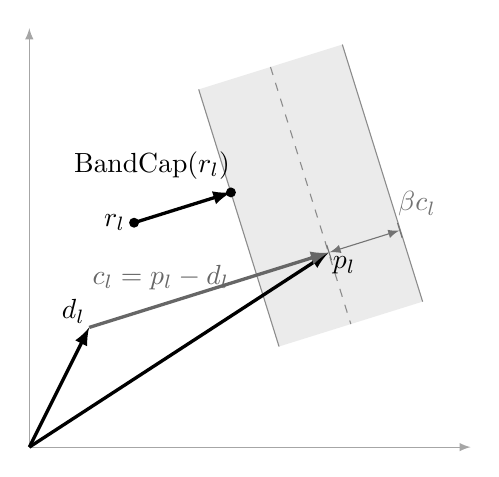
\begin{tikzpicture}[x=0.95cm, y=0.95cm, >=latex, line join=round]
    % Axes of the 2D slice.
    \draw[->, black!35] (0,0) -- (5.9,0);
    \draw[->, black!35] (0,0) -- (0,5.6);

    % The band: a slab perpendicular to c_l, centred on p_l's projection.
    \fill[black!8] (2.264,4.782) -- (4.184,5.382) -- (5.258,1.945) --
                   (3.338,1.345) -- cycle;
    \draw[black!45] (2.264,4.782) -- (3.338,1.345);
    \draw[black!45] (4.184,5.382) -- (5.258,1.945);
    % Centre line of the band: p_l's own projection on \hat c_l.
    \draw[dashed, black!45] (3.224,5.082) -- (4.298,1.645);

    % The two published vectors and their difference.
    \draw[->, very thick] (0,0) -- (0.8,1.6) node[above left, inner sep=1pt] {$d_l$};
    \draw[->, very thick] (0,0) -- (4.0,2.6) node[below right, inner sep=1pt] {$p_l$};
    \draw[->, very thick, black!60] (0.8,1.6) -- (4.0,2.6)
      node[pos=0.3, above, inner sep=5pt, black!60] {$c_l = p_l - d_l$};

    % Half-width of the band, measured along \hat c_l from p_l.
    \draw[|<->|, black!55] (4.0,2.6) -- (4.96,2.90);
    \node[black!55, anchor=west, inner sep=2pt] at (4.85,3.25)
      {$\beta \lVert c_l \rVert$};

    % A residual stream activation short of the band, moved to the near edge.
    \fill (1.4,3.0) circle (1.8pt) node[left, inner sep=3pt] {$r_l$};
    \draw[->, very thick] (1.4,3.0) -- (2.695,3.405);
    \fill (2.695,3.405) circle (1.8pt);
    \node[anchor=south east, inner sep=3pt] at (2.80,3.46)
      {$\mathrm{BandCap}(r_l)$};
  \end{tikzpicture}
  \caption{Band-capping in a 2D slice of the residual stream. The persona
  vector $p_l$ and the default vector $d_l$ define the diff direction
  $c_l = p_l - d_l$. The shaded slab is the band: the activations whose
  projection on $\hat{c}_l$ falls within $\beta \lVert c_l \rVert$ of $p_l$'s,
  so its edges run perpendicular to $c_l$ and the dashed line marks $p_l$'s own
  projection. An activation $r_l$ short of the band is moved parallel to
  $\hat{c}_l$ onto the near edge, which leaves its component orthogonal to
  $\hat{c}_l$ untouched; activations already inside the slab are left alone.}
  \label{fig:steering-geometry}
\end{figure}
; needs tikz and amsmath.
\begin{figure}[t]
  \centering
  \footnotesize
  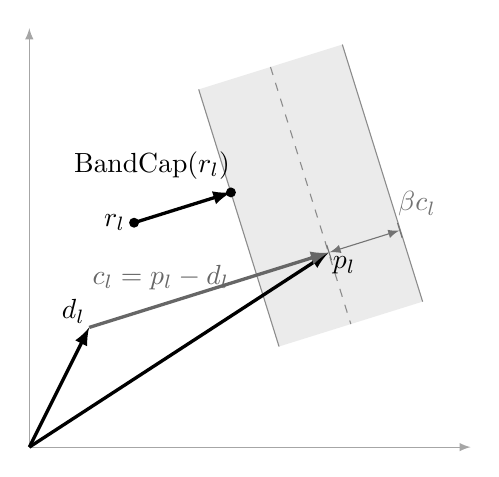
\begin{tikzpicture}[x=0.95cm, y=0.95cm, >=latex, line join=round]
    % Axes of the 2D slice.
    \draw[->, black!35] (0,0) -- (5.9,0);
    \draw[->, black!35] (0,0) -- (0,5.6);

    % The band: a slab perpendicular to c_l, centred on p_l's projection.
    \fill[black!8] (2.264,4.782) -- (4.184,5.382) -- (5.258,1.945) --
                   (3.338,1.345) -- cycle;
    \draw[black!45] (2.264,4.782) -- (3.338,1.345);
    \draw[black!45] (4.184,5.382) -- (5.258,1.945);
    % Centre line of the band: p_l's own projection on \hat c_l.
    \draw[dashed, black!45] (3.224,5.082) -- (4.298,1.645);

    % The two published vectors and their difference.
    \draw[->, very thick] (0,0) -- (0.8,1.6) node[above left, inner sep=1pt] {$d_l$};
    \draw[->, very thick] (0,0) -- (4.0,2.6) node[below right, inner sep=1pt] {$p_l$};
    \draw[->, very thick, black!60] (0.8,1.6) -- (4.0,2.6)
      node[pos=0.3, above, inner sep=5pt, black!60] {$c_l = p_l - d_l$};

    % Half-width of the band, measured along \hat c_l from p_l.
    \draw[|<->|, black!55] (4.0,2.6) -- (4.96,2.90);
    \node[black!55, anchor=west, inner sep=2pt] at (4.85,3.25)
      {$\beta \lVert c_l \rVert$};

    % A residual stream activation short of the band, moved to the near edge.
    \fill (1.4,3.0) circle (1.8pt) node[left, inner sep=3pt] {$r_l$};
    \draw[->, very thick] (1.4,3.0) -- (2.695,3.405);
    \fill (2.695,3.405) circle (1.8pt);
    \node[anchor=south east, inner sep=3pt] at (2.80,3.46)
      {$\mathrm{BandCap}(r_l)$};
  \end{tikzpicture}
  \caption{Band-capping in a 2D slice of the residual stream. The persona
  vector $p_l$ and the default vector $d_l$ define the diff direction
  $c_l = p_l - d_l$. The shaded slab is the band: the activations whose
  projection on $\hat{c}_l$ falls within $\beta \lVert c_l \rVert$ of $p_l$'s,
  so its edges run perpendicular to $c_l$ and the dashed line marks $p_l$'s own
  projection. An activation $r_l$ short of the band is moved parallel to
  $\hat{c}_l$ onto the near edge, which leaves its component orthogonal to
  $\hat{c}_l$ untouched; activations already inside the slab are left alone.}
  \label{fig:steering-geometry}
\end{figure}
; needs tikz and amsmath.
\begin{figure}[t]
  \centering
  \footnotesize
  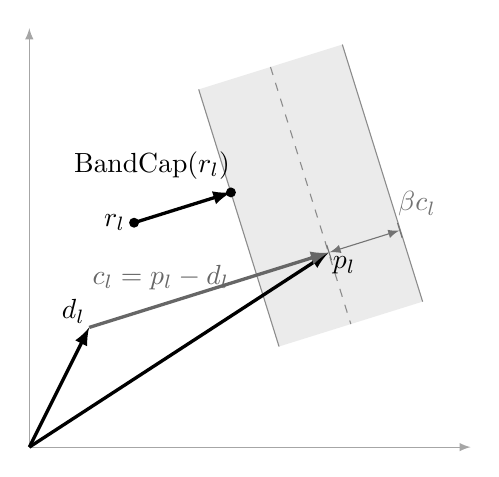
\begin{tikzpicture}[x=0.95cm, y=0.95cm, >=latex, line join=round]
    % Axes of the 2D slice.
    \draw[->, black!35] (0,0) -- (5.9,0);
    \draw[->, black!35] (0,0) -- (0,5.6);

    % The band: a slab perpendicular to c_l, centred on p_l's projection.
    \fill[black!8] (2.264,4.782) -- (4.184,5.382) -- (5.258,1.945) --
                   (3.338,1.345) -- cycle;
    \draw[black!45] (2.264,4.782) -- (3.338,1.345);
    \draw[black!45] (4.184,5.382) -- (5.258,1.945);
    % Centre line of the band: p_l's own projection on \hat c_l.
    \draw[dashed, black!45] (3.224,5.082) -- (4.298,1.645);

    % The two published vectors and their difference.
    \draw[->, very thick] (0,0) -- (0.8,1.6) node[above left, inner sep=1pt] {$d_l$};
    \draw[->, very thick] (0,0) -- (4.0,2.6) node[below right, inner sep=1pt] {$p_l$};
    \draw[->, very thick, black!60] (0.8,1.6) -- (4.0,2.6)
      node[pos=0.3, above, inner sep=5pt, black!60] {$c_l = p_l - d_l$};

    % Half-width of the band, measured along \hat c_l from p_l.
    \draw[|<->|, black!55] (4.0,2.6) -- (4.96,2.90);
    \node[black!55, anchor=west, inner sep=2pt] at (4.85,3.25)
      {$\beta \lVert c_l \rVert$};

    % A residual stream activation short of the band, moved to the near edge.
    \fill (1.4,3.0) circle (1.8pt) node[left, inner sep=3pt] {$r_l$};
    \draw[->, very thick] (1.4,3.0) -- (2.695,3.405);
    \fill (2.695,3.405) circle (1.8pt);
    \node[anchor=south east, inner sep=3pt] at (2.80,3.46)
      {$\mathrm{BandCap}(r_l)$};
  \end{tikzpicture}
  \caption{Band-capping in a 2D slice of the residual stream. The persona
  vector $p_l$ and the default vector $d_l$ define the diff direction
  $c_l = p_l - d_l$. The shaded slab is the band: the activations whose
  projection on $\hat{c}_l$ falls within $\beta \lVert c_l \rVert$ of $p_l$'s,
  so its edges run perpendicular to $c_l$ and the dashed line marks $p_l$'s own
  projection. An activation $r_l$ short of the band is moved parallel to
  $\hat{c}_l$ onto the near edge, which leaves its component orthogonal to
  $\hat{c}_l$ untouched; activations already inside the slab are left alone.}
  \label{fig:steering-geometry}
\end{figure}
